\chapter{Analyse}
\label{ch:analysis}

\section{Wettbewerbsanalyse}
\label{sec:competitionanalysis}
% \section{Wettbewerbsanalyse}

Das Ermitteln und Priorisieren aller relevanten Kundenanforderungen ist ein kontinuierlicher und unerlässlicher Vorgang, um zum einen die Bedürfnisse der zukünftigen Nutzer erfüllen zu können und zum anderen, um das Produkt langfristig wettbewerbsfähig zu gestalten. Hierfür ist es essenziell, sich mit Wettbewerbern, ihren Produkten und vermeintlichen Strategien auseinandersetzten. Erst dies bildet die Grundlage die eigenen Chancen auf dem Markt zu bewerten und mögliche Alleinstellungsmerkmale (\engl unique selling point, USP) zu ermitteln, um sich von Wettbewerbern frühzeitig abzusetzen. Zusätzlich zeigt die Analyse, welche Features bereits auf dem Markt im Einsatz sind und vom User \ggf schon als grundlegende Features erwartet werden.

Die Durchführung der Wettbewerbsanalyse erfolgte in den folgenden Einzelschritten:

\begin{itemize}
    \item Ermittlung der Hauptwettbewerber
    \item Erstellung eines Konkurrenzprofils
    \item Darstellung der einzelnen Wettbewerber
    \item Bewertung der strategischen Ausrichtung
    \item Zusammenfassung
\end{itemize}

\subsection{Ermittlung der Hauptwettbewerber}

Für die Ermittlung der bedeutendsten Mitbewerber ist es erforderlich die Hauptmerkmale und Ziele des eigenen Dienstes, für einen Abgleich mit den potenziellen Wettbewerbern, gut zu kennen. Hierbei ist zu berücksichtigen, dass es in der digitalen Welt selten Wettbewerber gibt, die 1:1 den gleichen Dienst anbieten \bzw die gleiche Strategie verfolgen. Jedoch können hierbei mittelfristig vollwertige Konkurrenzprodukte entstehen, die zum Zeitpunkt der Analyse nur wenige gemeinsame Parallelen oder Features aufgewiesen haben.

Digital Home Town (DHT) setzt in seiner langfristigen Ausrichtung auf die Stärkung des lokalen/ regionalen Raums mit seinen sozialen Verflechtungen. Dies soll geschehen durch die Förderung des digitalen Austauschs zwischen allen Menschen und Institutionen, die das örtliche Dasein widerspiegeln. Die Schwerpunkte von DHT sind wie folgt:

\begin{enumerate}
    \item Das Vernetzen von Personen, die das gleiche Interesse oder ähnliche Bedürfnisse teilen, einen Austausch von \bspw Informationen, Waren \usw anstreben oder Unterstützung/ Hilfestellung suchen.
    \item Die Stärkung lokaler Vereine und/ oder Dienstleistungen, damit diese ihre Angebote gezielter darstellen und leichter mit Interessierten in Kontakt treten können.
    \item Die Unterstützung öffentlicher Einrichtungen, um einen leichteren Zugang \ua zu amtlichen Informationen, Terminen \usw zu ermöglichen.
\end{enumerate}

Zugleich sieht sich DHT allen Personen verpflichtet und strebt einen barrierefreien Zugang an.

Abgeleitet aus der Zielsetzung von DHT konnten eine Reihe von Web-Diensten ermittelt werden, die sich \ua auf den lokalen Raum in Bezug auf Austausch, Vernetzung oder Zusammenführung privater Parteien konzentrieren. Als besonders etablierte und aktive Vertreter in mindestens einem der genannten Bereiche konnten zunächst

\begin{itemize}
    \item Facebook,
    \item Nebenan.de,
    \item Spontacts,
    \item eBay Kleinanzeigen und
    \item Doctolib
\end{itemize}

ausfindig gemacht werden. Im weiteren Verlauf werden exemplarisch nur die Social-Networking-Vertreter weiter ausgeführt. Dies betrifft demnach nicht Doctolib, da es sich eher um eine spezialisierte Software für E-Health-Angebote handelt.

\subsection{Konkurrenzprofil}

Zur detaillierten Auseinandersetzung mit den ermittelten Wettbewerbern ist es erforderlich ein Profil jedes einzelnen zu erstellen. Dieses sogenannte Konkurrenzprofil gibt in der Gegenüberstellung mit dem eigenen Selbstprofil eine transparente Bewertungsbasis, mit dessen Hilfe wertvolle Erkenntnisse über die Stärken, Potenziale und strategischen Ziele abgeleitet werden können.

Für den Vergleich werden die folgenden Punkte gesondert betrachtet:

\begin{itemize}
    \item Fokus des Dienstes und dessen Zielgruppe,
    \item Möglichkeiten der Selbstdarstellung und des Austausches,
    \item Benachrichtigungen über Änderungen und Neuigkeiten und
    \item Entdecken von Inhalten.
\end{itemize}

\subsection{Kurzdarstellung}

\subsubsection{Facebook}

Facebook ist ein etablierter und weltweit verbreiteter Dienst, der es ermöglicht sich mit Menschen aus der ganzen Welt zu vernetzen, miteinander in Kontakt zu bleiben und Inhalte aus dem eigenen Leben mit anderen zu teilen.
In den frühen Jahren von Facebook waren insbesondere Studenten die anvisierte Zielgruppe, welche über die Jahre jedoch breiter geworden und mittlerweile sehr heterogen ist.

\begin{figure}
    \centering
    \includegraphics[width=\textwidth]{figures/jan/pic_facebook.png}
    \caption[Startseite von Facebook]{Startseite von Facebook}
    \label{fig:facebook}
\end{figure}

Die Nutzung von Facebook kann je nach Bedürfnissen des Einzelnen sehr verschieden sein. Hier bietet Facebook neben reinen Darstellungs- und Austauschmöglichkeiten eine Bandbreite an Anwendungen an, wie \ua integrierte Video-, Games- und Dating-Portale und ein eigenes Bezahlsystem, auf welche hier im weiteren Verlauf nicht weiter eingegangen wird.

\paragraph{Selbstdarstellung}

Zur Darstellung einer Organisation, einer öffentlichen oder privaten Person, bietet Facebook je nach Typ ein eigenes Profil an, auf welchem \ua Bilder, persönliche Informationen und Vorlieben, wie \zB Musik öffentlich dargestellt werden können. Inwieweit diese Inhalte einsehbar sind, ist individuell einstellbar. Zusätzlich zu den statischen Informationen beinhaltet das Profil noch eine Pinnwand, auf welcher ältere und aktuelle Beiträge listenmäßig aufgeführt sind.

\paragraph{Formen des Austausches}

Für den interaktiven Austausch und das Teilen von Momenten dienen Beiträge (Posts) . Diese können von jedem verfasst und auf der eigenen sowie fremden Pinnwand angebracht werden. Diverse Ereignisse, wie \bspw das Hochladen von neuen Bildern, generieren systematisch einen eigenen Beitrag, um Bekannte, Follower \etc über eine Neuigkeit auf dem Profil zu informieren. Die Beiträge können wiederum von Anderen kommentiert oder mittels eines Icons bewertet werden. Zudem können sie neben einfachem Text auch Bilder oder Videos enthalten und lassen sich mittels Tags (Orte, GPS, Veranstaltungen, Personen, \ldots) genauer spezifizieren.

Für den Austausch mit mehreren Personen bietet Facebook Gruppen an. Dort können sich Anwender über gemeinsame Themen austauschen. Gruppen haben wie Profile einen statischen Teil, in dem die Admins im Freitext eine Kurzbeschreibung der Gruppe verfassen und veröffentlichen können. Darüber hinaus verfügen Gruppen auch über eine Pinnwand, über die die Mitglieder miteinander im Austausch stehen. Gruppenmitglieder können darüber hinaus auch Events erstellen, an welchen die Mitglieder teilnehmen können.
Gruppen werden sehr häufig und für verschiedene Themen verwendet. Sie dienen besonders im städtischen Raum \bspw zum Verschenken von ungenutzten Dingen (Free your Stuff), zum Finden von neuen Kontakten in einer neuen Stadt (New in Munich) oder das Finden von Menschen in der Nähe mit ähnlichen Hobbies (\zB Wandern). Auch der überregionale/ internationale Austausch über diverse Themen in unterschiedlichen Bereichen ist weit verbreitet.

Der Austausch materieller Gegenstände findet neben den einzelnen Gruppen hauptsächlich auf einem digitalen Marktplatz statt. Die geschalteten Anzeigen enthalten eine Überschrift, freie Beschreibungen, Bilder, Angaben über den Zustand, Preisvorstellung, Ort und den Herausgeber der Anzeige. Bei der Erstellung dieser muss der Verfasser die Anzeige einer vordefinierten Kategorie zuweisen, um die Auffindbarkeit zu erleichtern. Für den Interessenten besteht neben der direkten Kontaktaufnahme die Möglichkeit sich die Anzeige zu merken, sie mit einem Kontakt zu teilen oder einen Alarm zu erstellen, sobald ähnliche Produkte angeboten werden.

Zur Pflege von Kontakten ist es in Facebook möglich, Personen bei gegenseitigem Einverständnis in eine Kontaktliste aufzunehmen. Mithilfe dieser sogenannten Freundesliste können Inhalte selektiv verteilt werden. Für Personen, die nicht in der Kontaktliste enthalten sind, sind diese Inhalte nicht sichtbar. Darüber hinaus werden befreundete Personen über das Dashboard gezielter informiert, sobald ein Kontakt aus der Liste eine Aktivität durchgeführt hat.

Für den direkten und nicht öffentlichen Austausch wird dem Anwender ein Chat angeboten, in welchem 1:1- und Gruppenchats stattfinden können. Der Nachrichtenaustausch findet hierbei in Echtzeit statt. Die Nachrichten können analog, wie Beiträge, die gleichen Inhalte aufweisen (Bilder, Links \etc). In 1:1-Gesprächen ist es darüber hinaus auch möglich, Sprach- und Videoanrufe zu tätigen.

\paragraph{Neuigkeiten}

Um bei der Vielzahl der Beiträge und Reaktionen von Freunden oder in Gruppen den Überblick zu behalten, werden auf einem Dashboard Neuigkeiten in Form einer endlosen und unsortierten Liste angezeigt. Darüber hinaus beinhaltet das Dashboard kommerzielle Werbung und Beiträge von noch nicht abonnierten Gruppen, die für den Nutzer von Interesse sein könnten.

Neben dem Dashboard gibt es zusätzlich noch eine Notifications-Seite, welche einen gezielteren Fokus aufs Wesentliche ermöglicht. Notifications sind kurze Benachrichtigungen, die gesammelt in einer Liste abgelegt werden. Sie beinhalten \ua Geburtstage der Kontakte, bevorstehende angemeldete Events, neue Beiträge aus abonnierten Gruppen sowie Reaktionen auf eigene oder kommentierte Beiträge.

\paragraph{Recherche}

Zur Findung von Personen, Gruppen \usw existiert eine Suchfunktion, mit deren Hilfe alle FB-Inhalte durchsucht werden können. Mit dem Suchfilter können auch die Art der Inhalte, Verfasser, Gruppen, Zeitraum \uvm genauer spezifiziert werden.

Das Sichern von Beiträgen und öffentlichen Profilen kann ebenso vorgenommen werden. Das Speichern erfolt direkt am Objekt.
Gespeicherte Beiträge und öffentliche Profile können im Anschluss auf einer separaten Seite je nach Typ aufgelistet und dort auch verwaltet werden.

\subsubsection{Nebenan.de}

Nebenan.de ist ein im Jahr 2015 in Betrieb genommenes Portal, welches wie Facebook seinen Mehrwert im Vernetzen von Menschen sieht. Anders als Facebook fokussiert es sich dabei ausschließlich auf die unmittelbare Nachbarschaft des Anwenders.

\begin{figure}
    \centering
    \includegraphics[width=\textwidth]{figures/jan/pic_nebenan.png}
    \caption[Startseite von nebenan.de]{Startseite von nebenan.de}
    \label{fig:nebenan}
\end{figure}

Die Zielgruppe besteht daher aus allen in der Nachbarschaft vorkommenden Interessengruppen, wie \zB Bewohner, Vereine, Firmen und Organisationen. Die Nachbarschaftsgrenze wird durch die eigene Adresse vom System definiert und kann nicht individuell angepasst werden. Ein Austausch über die Nachbarschaftsgrenze hinaus ist nicht möglich, was den Fokus auf die Stärkung und Belebung der Nachbarschaft deutlich hervorhebt.

\paragraph{Selbstdarstellung}

Für die Darstellung existieren in Nebenan.de zwei Arten von Profilen. Die erste Profilart gilt Einzelnutzern. Hierbei können sich Anwohner über ein Kurzprofil mit Foto, einem Freitext sowie ihren Interessen und Angeboten vorstellen. Zur Auswahl der Interessen und Angebote stehen fest definierte Vorschläge zur Verfügung. Angebote beschreiben neben den Interessen, was der Anwohner bereit ist, in seine Nachbarschaft einzubringen. Dies könnte \bspw Pakete annehmen, Blumen gießen, Fahrrad reparieren oder Gesellschaft leisten sein.
Neben der eigenen Darstellung zeigt das Profil die Aktivität des Anwohners an. Dies beinhaltet \bspw die Auflistung von beigetretenen nebenan-Gruppen und die Anzahl der erhaltenen virtuellen Dankeschöns.
Die zweite Profilart wird von Organisationen und Läden/ Services genutzt, die vor Ort angesiedelt sind und zum alltäglichen Leben in der Nachbarschaft beitragen. Diese Profile sind im Vergleich zu den Anwohnerprofilen mit deutlich mehr Informationen ausgestattet. Jedes dieser Profile muss beim Anlegen mit einer Kategorie versehen werden. Dies kann im Beispiel eines Geschäftes \zB Restaurant, Reisen oder Sport und im Fall einer Organisation Non-Profit, Political Party, Nachbarschafts-Initiative \usw sein. Neben Name, Adresse, Kontaktdaten und Öffnungszeiten können auch zukünftige Ereignisse/ Events, Gesuche, Bekanntmachungen, das Verkaufsangebot und weitere Informationen hinterlegt werden. Die Anwohner können darüber hinaus ihre eigenen Erfahrungen mit der Organisation oder dem Laden sowie Empfehlungen auf deren öffentlichen Profilen kundtun.

\paragraph{Formen des Austausches}

Als zentrales Mittel für den Austausch wird bei nebenan.de der Beitrag genutzt. Dieser kann nach dem Veröffentlichen von allen Anwohnern kommentiert und positiv bewertet werden. Ein Beitrag wird bei der Erstellung mit einer Kategorie versehen. Anhand dieser wird festgelegt, ob es sich bei dem Beitrag um etwas Allgemeines, ein Gesuch, ein Angebot, eine Empfehlung oder ein Event handelt. Jede Kategorie wird des Weiteren zur besseren Einordnung noch in eine oder mehrere aufeinander aufbauende Unterkategorien unterteilt. Je nach Art werden die Beiträge neben der öffentlichen Wand zusätzlich an diverse Seiten wie \zB den Event-Feed im Marktplatz der Nachbarschaft angeheftet.
Die Beiträge bestehen wie bei Facebook klassisch aus einem Titel und einem Freitext und können optional mit Bildern versehen werden. Zusätzlich können je nach Art noch weitere Felder wie \zB Datum und Ort bei Veranstaltungen vorhanden sein.

Die Beiträge des Marktplatzes werden neben der Kategorie Angebot noch in die Unterkategorien Help, Give, Rent, Trade \usw unterteilt. Der Inhalt eines Verkaufsangebots kann des Weiteren noch mit einer Angebotskategorie, wie Food, Baby \& Children, Pets \usw, versehen werden. Alle Angebote werden gesammelt in einer Liste dargestellt und können nach ihrer Angebotskategorie gefiltert oder mit der globalen nebenan.de-Suchfunktion nach Wörtern durchsucht werden.

Für den Austausch von Personen mit gleichen Interessen können in nebenan.de Gruppen erstellt werden, deren Zweck durch einen Gruppennamen und einen Freitext genauer ausgeführt werden kann. In den Gruppen können verschiedene Arten von Beiträgen (Mitteilung, Suche, Angebot, Veranstaltung, \ldots) abgesetzt werden. Diese werden an der Gruppenpinnwand angezeigt und können von allen Gruppenmitglieder kommentiert werden. Die Gruppenfunktion findet jedoch auf nebenan.de nur eine geringe Beachtung.

Eine Chatfunktion für den direkten Austausch mit einzelnen Nutzern ist ebenso integriert. Neben dem reinen Text und Emoticons können mit ihr zusätzlich noch Fotos und Empfehlungen versandt werden.

\paragraph{Neuigkeiten}

Zur Benachrichtigung von neuen Beiträgen gibt es das Dashboard. Hier werden alle Arten von Beiträgen mit Ausnahme der Angebotsbeiträge (Give) nach der letzten Änderung sortiert angezeigt. Der Austausch mit der Nachbarschaft passiert maßgeblich über das Dashboard, wo reinkommende Beiträge entdeckt und beantwortet werden können.
Für den besseren Überblick werden durch Benachrichtungs alle Beiträge, bei denen man selbst aktiv teilgenommen hat und sich neue Ereignisse ergeben haben, nochmal separat aufgelistet.. Darüber hinaus werden auf dem Benachrichtungs-Feed alle Events angezeigt, die zukünftig in der Nachbarschaft stattfinden.

\paragraph{Recherche}

Für die Suche von Beiträgen jeglicher Art steht die nebenan-Suche zur Verfügung. Über diese können anhand eines Freitextes die Beiträge der Nachbarschaft durchforscht werden.
Beiträge, die dem User besonders zusagen oder für ihn wichtige Informationen enthalten, können als Bookmark gespeichert werden und auf der Bookmark-Seite unter Feed oder Marktplatz eingruppiert eingesehen und wieder gelöscht werden.

\subsubsection{Spontacts}

Gegenüber Facebook und Nebenan.de legt Spontacts sein Augenmerk ausschließlich auf das Verabreden/ Treffen für Freizeitaktivitäten von Menschen, die in der gleichen Region wohnen. Spontacts richtet sich an Menschen, die Interesse an bestimmten Aktivitäten haben und dazu neue Kontakte suchen.

\begin{figure}
    \centering
    \includegraphics[width=\textwidth]{figures/jan/pic_spontacts.png}
    \caption[Startseite von Spontacts]{Startseite von Spontacts}
    \label{fig:spontacts}
\end{figure}

Der Anwender kann hierfür an erstellten Veranstaltungen teilnehmen oder selbst welche erstellen. Im Gegensatz zu den bereits vorgestellten Diensten besitzt Spontacts einen kostenlosen sowie kostenpflichtigen Account. Ein weiterer Unterschied liegt darin, dass regelmäßig Angebote für die Nutzer von bei Spontacts Angestellten bereitgestellt werden und es sich dadurch nicht um reinen User-Content handelt.

\paragraph{Selbstdarstellung}

Die Benutzer von Spontacts können, wie auch in vergleichbaren Anwendungen, zur Präsentation ihrer Person ein Profil erstellen. Das Grundprofil setzt sich aus Name, Profilbild, Alter und Wohnort zusammen und kann mit weiteren Informationen wie \bspw präferierte Kontakte - für Freizeit, Sport, Reisen, Tanzen und Dating - oder mit zusätzlichen Profilabschnitten (Hobbies, Interessen/ Vorlieben \usw) angereichert werden. In einem weiteren Abschnitt können vergangene und zukünftige Aktivitäten des Users sowie seine Gruppenmitgliedschaften eingesehen werden.

\paragraph{Formen des Austausches}

Zur Interaktion mit anderen Benutzern dienen Beiträge. Diese Beiträge werden je nach Art als einfacher Beitrag, als Aktivität oder als Frage/ Diskussion abgesetzt und anschließend in Communities, Gruppen oder \ggf in Foren angezeigt und können wie gewohnt kommentiert, gelikt und geteilt werden.

Die Communities beschreiben als eine Obergruppe einen Themenbereich (Ausgehen \& Party, Essen \& Trinken, Natur \& Umwelt \usw), zu welchem der Beitrag zugeordnet wird. Beim Erstellen einer Gruppe muss hierfür immer eine passende Community ausgewählt werden.
Anders als bei den anderen vorgestellten Diensten, stellen die Gruppen auf Spontacts das zentrale Feature der Anwendung dar. Diese ähneln vom Funktionsumfang den FB-Gruppen und sind lediglich in ihrem Aufbau anders strukturiert. In ihnen kann sich der Anwender über das Gruppenprofil mit Kurzbeschreibung, Mitgliederanzahl \usw informieren, über eine Pinnwand alle Beiträge der Mitglieder durchstöbern sowie die geplanten Veranstaltungen der Gruppe einsehen.

Für Auseinandersetzungen über die Beiträge hinaus kann mit jedem Anwender eine private Unterhaltung über den Chat geführt werden. Mit dem Chat können Textnachrichten ohne Emoticons, Bilder \etc versendet werden.

\paragraph{Recherche}

Zum Entdecken von Beiträgen, Veranstaltungen, Gruppen, Mitgliedern \uvm bietet eine Suchfunktion je nach zu suchendem Typ weitere Filterfunktionen. Der Anwender kann neben den allgemeinen Einstellungen wie Suchbegriff, Umkreis, Erstelldatum und Community die Anfrage noch mit objektspezifischen Kriterien wie Datum, Alter und ähnliches verfeinern.

Die während der Nutzung des Portals oder während eines Treffens entdeckten Mitglieder können in die Kontaktliste oder Merkliste aufgenommen werden. Die Merkliste ist eine private Liste von Personen, die der Anwender als merkenswert empfand. Die Kontaktliste ist hingegen öffentlich und zur Aufnahme muss eine Anfrage an die Person versendet und bestätigt werden.
Darüber hinaus kann man Mitgliedern folgen, um ihre Aktivitäten besser verfolgen zu können. Wer wem folgt kann jeder Benutzer im jeweiligen Profil einsehen.

\paragraph{Neuigkeiten}

Um innerhalb der Plattform auf dem Laufenden zu bleiben, gibt es wie bei den anderen Portalen ein Dashboard und einen Benachrichtigungs-Feed.
Im Dashboard werden in der Rubrik „Neuigkeiten“ alle anstehenden Veranstaltungen und aktuellen Inhalte aus den gewählten Communities dargestellt. Unter der Rubrik \glqq Mein Feed\grqq\ im Dashboard können
hingegen alle Veränderungen in beigetretenen Gruppen eingesehen werden. Hierzu zählen insbesondere neue Mitglieder und neue Veranstaltungen.
Der Benachrichtungs-Feed enthält neue Kontaktanfragen, Beiträge aus den Gruppen und Plattform News.

\subsection{Strategische Ausrichtung}

Die drei untersuchten Hauptwettbewerber weisen als soziale Netzwerke insbesondere in ihren Features, wie das Vorhandensein von Profil, Chat, Gruppen \usw, viele Gemeinsamkeiten auf. In ihrer strategischen Ausrichtung unterscheiden sie sich jedoch teils stark voneinander.
Facebook ist eine sehr aktive Plattform. Sie unterstützt ganz allgemein das Vernetzen von Menschen mit beliebigen Interessen, Themen und Bedürfnissen. Es fokussiert sich dabei nicht auf einen geografischen Raum oder schränkt die Anwender in irgendeiner Form ein, die einen Austausch verhindern würde. Ein Ausbau oder eine intensive Weiterentwicklung an der Plattform konnte in der vergangenen Zeit nicht wahrgenommen werden \bzw dieser fand nur im Hintergrund statt. Lang- und mittelfristig ist hierbei keine Veränderung zu erwarten, da sich der Konzern hinter Facebook maßgeblich der Entwicklung von zukünftigen Produkten im 3D-Umfeld gewidmet hat.

Nebenan.de ist in seiner bisherigen Ausrichtung der größte Konkurrent für DHT. Die Plattform bietet die Möglichkeit sich innerhalb der eigenen Nachbarschaft zu verschiedenen Themen auszutauschen und zu vernetzen. Der Fokus liegt hierbei auf der Stärkung des Miteinanders in einem lokalen Raum. Die große Herausforderung, die vor Nebenan.de liegt, ist maßgeblich der Aufbau von lokalen Communities, in welchen sich alle gesellschaftlichen Schichten und Altersklassen angesprochen fühlen. Ein weiteres Vorhaben könnte zugleich auch der Ausbau der Plattform sein, um zum einen diese intuitiver zu gestalten sowie zum anderen einen zielgerichteteren Austausch zu ermöglichen.

Spontacts fokussiert sich hingegen sehr stark auf das Vernetzen von Menschen zur Durchführung gemeinsamer Aktivitäten im privaten Bereich. Die Plattform hat eine rege Community. Die Anwender sind in der Lage beliebige Inhalte zu erstellen und an allen Veranstaltungen innerhalb Spontacts teilzunehmen. Harte lokale Einschränkungen \bzgl der Sichtbarkeit von Inhalten existieren wie auch bei nebenan.de nicht.
Die Inhalte der Seite werden darüber hinaus noch durch lokal ansässige Moderatoren betreut. Die Moderatoren erstellen ergänzend weitere Veranstaltungsangebote und führen diese zugleich auch durch. Strategisch versucht Spontacts zunehmend kostenpflichtige Accounts einzuführen, über welche zusätzliche Funktionen, wie \bspw bessere Filterfunktionen, den Anwendern zur Verfügung stehen. Ein weiterer Schritt, um sich weiter auf dem Markt zu etablieren, wäre es die bisherige Zielgruppe - alleinstehend und \ca 30-50 Jahre - zunehmend weiter anzusprechen.

\subsection{Zusammenfassung}

Mithilfe der durchgeführten Analyse der Wettbewerber konnte verdeutlicht werden, dass die untersuchten Dienste alle verschiedene Motivationen sowie Zielgruppen verfolgen. Zugleich verfolgt keiner den Ansatz sich, wie DHT, gezielt auf die Region/ Gemeinde zu konzentrieren, um dort die Vernetzung und den Austausch zu fördern. DHT schließt hierbei die Lücke, die sich zwischen FB als weltweiter Akteur und nebenan.de mit reinem Nachbarschaftsfokus auftut. Absetzen tut sich DHT neben dem örtlichen Bezug auch durch die Einbindung von Vereinen und öffentlichen Organen, die die Plattform zur Kommunikation mit den Anwohnern nutzen können.

Ein weiterer Aspekt, der im direkten Vergleich deutlich wird, ist, dass die Bedienung und das Zurechtfinden auf den Plattformen sehr unterschiedlich ausfallen. Teils sind die Inhalte sehr versteckt, teils sind die zugrunde liegenden Konzepte nicht selbsterklärend gestaltet. Durch den Anspruch von DHT für alle von jung bis alt (generationsübergreifend) verständlich zu sein, ist es essenziell für den Erfolg von DHT, eine Plattform zu entwerfen, die in der Handhabung einfach und intuitiv ist.

Die Analyse zeigt am Beispiel von nebenan.de und Spontacts auch, dass der Aufbau und das Etablieren eines sozialen Netzwerkes viele Herausforderungen mit sich bringen. Als Vorreiter ist Facebook sehr weit in der Gesellschaft verbreitet und ermöglicht durch sein breites Angebot an Features diese für verschiedene Bedürfnisse zu nutzen.
Dies stellt insbesondere neuere Plattformen - wie Nebenan.de und Spontacts - im Aufbau einer Community vor große Herausforderungen, da sie als Newcomer ohne Community und Content mit meist den gleichen FB-Features den Anwender überzeugen müssen, sodass ihre Plattform einen spürbaren Mehrwert gegenüber FB liefert. Dies ist besonders bei Plattformen schwierig, bei denen die Inhalte ausschließlich von den Nutzern erstellt werden. Der Aufbau einer solchen Community ist als besonders zäh anzusehen, da neue Nutzer sich aus Mangel an aktuellen Inhalten schnell wieder von der Plattform abwenden.
Das kontinuierliche Vorhandensein von neuen Inhalten ist ein essenzieller Bestandteil, um ein Etablieren zu ermöglichen. Spontacts setzt hierfür gezielt seine Moderatoren ein, um ein regelmäßiges Angebot für seine Nutzer zur Verfügung zu stellen. Alternativ kann die Bindung an ein Portal auch durch Angebote von Dritten erfolgen. Dies kann \bspw durch regelmäßige Informationen von Vereinen, einer Stadtverwaltung oder einer Zeitung stattfinden, wie für DHT angedacht, oder durch zusätzliche Funktionen, die den Nutzer bei bestimmten Dingen unterstützen, wie \zB ein Buchungsportal oder Ähnliches.


\section{Anforderungsanalyse}
\label{sec:requirementanalysis}
% \section{Requirementsanalysis}

Die Anforderungsanalyse ist ein entscheidender Schritt im Software-Entwicklungsprozess, der dazu beiträgt, die Bedürfnisse der Nutzer zu identifizieren und zu verstehen. Um jedoch die Bedürfnisse der Nutzer vollständig zu verstehen, ist es notwendig, eine detaillierte Analyse der Geschäftsanforderungen durchzuführen. Das Value Proposition Canvas bietet dabei eine effektive Methode zur Identifizierung der Kundenbedürfnisse und zur Entwicklung von wertvollen Produkten und Services. Dieses Kapitel befasst sich mit der Anforderungsanalyse mit dem Hilfsmittel des Value Proposition Canvas.

\subsection{Value Proposition Canvas}

Die Anforderungsanalyse nach dem Value Proposition Canvas ist ein Prozess, bei dem die Bedürfnisse und Anforderungen der Kunden identifiziert und dokumentiert werden, um sicherzustellen, dass das Unternehmen Produkte oder Dienstleistungen anbietet, die einen hohen Nutzen für die Kunden bieten.

\begin{figure}
    \centering
    \includegraphics[width=0.6\textwidth]{figures/andre/valuepropositioncanvas.jpg}
    \caption{Value Proposition Canvas}
    \label{fig:valuepropositioncanvas}
\end{figure}

Der Value Proposition Canvas besteht aus zwei Hauptbereichen:

\begin{itemize}
    \item[1.]	Der Kundenprofilbereich: In diesem Bereich identifizieren Sie die Bedürfnisse und Anforderungen Ihrer Zielgruppe und erstellen ein detailliertes Profil der Kundenperspektive.
    \item[2.]	Der Value-Map-Bereich: In diesem Bereich legen Sie fest, wie Ihr Produkt oder Ihre Dienstleistung den Kundenbedarf erfüllt und welche Vorteile es im Vergleich zu anderen Lösungen bietet.
\end{itemize}

\subsection*{Vorgehensweise}

Um eine erfolgreiche Analyse nach dem Value Proposition Canvas durchzuführen, sollten folgende Schritte beachtet werden:

\begin{itemize}
    \item[1.] Kundenprofilbereich 
    \begin{itemize}
        \item Identifizierung der Bedürfnisse und Herausforderungen der Zielgruppe
        \item Definierung der Kundenperspektive und Erstellen eines Profils für die Zielgruppe
    \end{itemize}
    \item[2.] Value-Map-Bereich
    \begin{itemize}
            \item Definition der Produkte oder Dienstleistungen, die angeboten werden sollen
            \item Festlegung der Vorteile, die das Produkt gegenüber anderen Konkurrenten bieten könnte
            \item Sicherstellung, dass die Bedürfnisse der Zielgruppe erfüllt werden
    \end{itemize}
\end{itemize}

\subsection{Personas und Zielgruppe}
Zu Beginn des Projekts wurde bereits die initiale Zielgruppe definiert. Da eine Social Media Plattform grundsätzlich ein potentiell sehr breites Spektrum an Nutzern besitzt, wurde die Entscheidung der Zielgruppe anhand dem bestmöglichen erreichen vieler Menschen definiert: Junge Erwachsene und Vereine - unter Betrachtung eines eher ländlicheren Landkreises.

Junge Erwachsene sind in der Regel affin und offener für den Umgang mit Technik, bei Erfolg der Plattform könnten diese wiederum über persönliche Kontakte und Werbung weitere Nutzer auf die Plattform ziehen. Vereine besitzen in der Regel bereits ein Netzwerk und bieten gleichzeitig die Möglichkeit, Menschen mit ähnlichen Interessen miteinander zu verknüpfen.

\subsection{Profile}
Um die Zielgruppen abbilden zu können, wurden insgesamt 4 Profile definiert, diese wurden nach dem Value Proposition Canvas analysiert und daraus jeweils Features abgeleitet. Diese sollen im Folgenden beschrieben werden:
\subsection*{Musikverein}
Beim Musikverein wird angenommen, es handelt sich um einen existierenden Verein mit einer funktionierenden Vorstandschaft und einer lebhaften Mitgliedschaft.
Dieser hat nach dem Value Proposition Design die folgenden Eigenschaften:


\subsection*{Alleinstehender Erwachsener Mann, frisch zugezogen}
Bei dieser Person handelt es sich um einen jungen alleinstehenden Mann, der erst wenige Wochen im Ort wohnt um eine neue Arbeit anzutreten. Dieser kennt nur das nötigste, ist zwar technikaffin, aber handwerklich nicht sonderlich begabt.

\subsection*{Alleinstehende Frau mittleren Alters}
Diese Frau ist alleinstehend, geschieden und Vollzeit berufstätig. Sie hat 2 jugendliche Kinder welche bei ihr wohnen und ist auf der Suche nach einem neuen Lebenspartner. Sie ist Mitglied in einem Gartenbauverein in der Gemeinde.

\subsection*{Junges Pärchen}
Mit diesem Profil soll ein junges Pärchen abgebildet werden. Diese sind beide Mitte 20 und leben in ihrer ersten gemeinsamen Wohnung. Beide sind voll berufstätig und daher zeitlich sehr eingeschränkt. Beide studieren und würden ihr wissen gerne mit anderen teilen.

\subsection{Abgeleitete Features}
Zusammen mit den Zielen aus der Aufgabenbeschreibung sowie den Erkenntnissen aus der Kundenanalyse des vorange-gangenen Kapitels wurden folgende Features abgeleitet.

\subsubsection{Persönliche und Vereinsprofile}
\label{sec:abgeleitetefeatures}
Im Vordergrund einer Social Media Plattform steht die Darstellung der eigenen Person. Daher war die Grundlage für die Plattform die Implementierung von Profilen.
Die Anforderungen für das Profil waren, sich kurz und knapp selbst beschreiben zu können. Die Einfachheit der Bedienung und damit für potentielle Profiländerungen sollte gegeben sein. Mit den Nutzerprofilen sollte nur das Interesse an der Person oder dem Verein geweckt werden, um im nächsten Schritt einen direkten Kontakt über die Chatfunktion zu ermöglichen.
Ein Schlüsselelement der Plattform ist das sogenannte Tag-System, ähnlich dem bekannten Hash-Tag von Netzwerken wie bspw. Twitter. Über die Tags kann ein Nutzer seine Hobbys und Interessenfelder kurz und knapp angeben.
Zusätzlich zum Tag sollte auch die Möglichkeit gegeben sein, sich selbst über einen Freitext beschreiben zu können.
Die Option ein Profilbild hochladen zu können ist ebenfalls eines der Basis-Anforderungen die das System haben muss.

\begin{figure}[ht!]
    \centering
    \includegraphics[width=0.6\textwidth]{figures/andre/beispielprofil.jpg}
    \caption{Beispielprofil}
    \label{fig:beispielprofil}
\end{figure}

In der obigen Abbildung ist ein Beispielhaftes Profil zu sehen. Es kann kurz und knapp auf das Thema der Organisation, in diesem Fall ein Fanclub über Arnold Schwarzenegger, abgeleitet werden. Des Weiteren sind auf dem Profil auch die erstellten Beiträge zu finden, ebenso wie eine Möglichkeit direkten Kontakt aufnehmen zu können. 

\subsubsection{Chats und Chaträume}
Ebenso obligatorisch wie die Profile ist auch die Chatfunktion, die zur Kontaktaufnahme unabdingbar ist. 
Auch hier stand wieder die Einfachheit im Fokus. Dies kann dadurch begründet werden, dass die Plattform nur zum Kennenlernen und Vernetzen der Menschen gedacht ist.
Ebenfalls soll die Möglichkeit bestehen, Gruppenchats zu erstellen. Dadurch kann man sowohl den Privatpersonen als auch Vereinen eine Möglichkeit geben sich in Gruppen zu organisieren. 

\begin{figure}[ht!]
    \centering
    \includegraphics[width=0.6\textwidth]{figures/andre/chatsundchaträume.jpg}
    \caption{Chats in Digital Dahoam}
    \label{fig:chatsundchaträume}
\end{figure}

\subsubsection{Beiträge, Veranstaltungen und Events}
Ebenfalls wichtig zur Kommunikation und Selbstdarstellung ist das Erstellen von Beiträgen. 

Aufgrund der Anforderungen wurden hierfür 4 Kategorien an Beiträgen herauskristallisiert:

\begin{itemize}
    \item	\textbf{Angebot} Man bietet etwas an, wie bspw. Hilfeleistung bei handwerklichen Tätigkeiten
    \item	\textbf{Anfrage} Hilfegesuch zu einem bestimmten Thema
    \item   \textbf{Information} Allgemeine Mitteilung
    \item 	\textbf{Veranstaltung} Teilen einer bevorstehenden Veranstaltung
\end{itemize}

Durch diese Kategorien können grundlegend die meisten Bedürfnisse zufriedengestellt werden. Es gibt sowohl die Möglichkeit, sich auszutauschen, als auch die Möglichkeit aktiv bzw. passiv nach Hilfe in der Nachbarschaft zu suchen bzw. diese anzubieten. Vereine können ihre Events mit der Öffentlichkeit teilen.

\subsubsection{Marktplatz und Entdecken}

Aufbauend auf den Beiträgen soll der Nutzer die Möglichkeit haben, gezielt nach eben jenen suchen zu können. Dies soll über das Explorationstool der Website ermöglicht werden.
Die Anforderungen hierfür waren, dass grundsätzlich nach allem und jedem gesucht bzw. gefiltert werden kann, anhand der zugewiesenen Tags. Dadurch kann dem Nutzer ermöglicht werden, auch wirklich nur die Beiträge zu sehen, die ihn auch Interessieren.
Des Weiteren sollten basierend auf demselben Prinzip (Tags) auch Personen gefunden werden können. Es wurde hierbei bewusst auf eine Klarnamensuche verzichtet, mit dem Ziel so möglichst viele neue Bekanntschaften zu ermöglichen. 

\begin{figure}[h!]
    \centering
    \includegraphics[width=0.6\textwidth]{figures/andre/marktplatzvondigitaldahoam.jpg}
    \caption{Marktplatz von Digital Dahoam}
    \label{fig:marktplatzvondigitaldahoam}
\end{figure}

\subsubsection{Persönlicher Merkzettel}
Als weiteres Feature sollte ein sog. Merkzettel implementiert werden. Dieser stellte sich als unabdingbar notwendig heraus für den Fall, dass ein Nutzer eine Veranstaltung sieht an der er interessiert ist und für später merken möch-te.
Aus dieser Anforderung wurde das allgemeine Feature des Merkzettels implementiert, sodass grundsätzlich die Möglichkeit gegeben ist, sich alle Beiträge merken zu können. Ähnlich wie beim Marktplatz kann auch hier nach den verschiedenen Beitragstypen gefiltert werden.

\begin{figure}[ht!]
    \centering
    \includegraphics[width=0.6\textwidth]{figures/andre/merkzettel.jpg}
    \caption{Merkzettel}
    \label{fig:merkzettel}
\end{figure}

\section{Visuelle Grundstrukturen}
\label{sec:visualstructure}
% \section{Visuelle Grundstrukturen}

Ein wichtiger Faktor für den Erfolg des Scrum-Teams ist es, dass jeder im Team das gleiche Verständnis über das zu entwickelnde Produkt hat. Die Sicherstellung dessen ist von hoher Bedeutung, um vermeidbaren Zeitfressern, wie lange Diskussionen, Missverständnisse, Nacharbeit und eine \ggf daraus hervorgehende Demotivation im Team entgegenzuwirken.
Darüber hinaus entstehen durch eine Visualisierung des Produktes Ideen und Lösungsansätze für Abläufe und Features, die frühzeitig im Entwicklungsprozess angesprochen, diskutiert und eingearbeitet werden können, ohne einen bemerkbaren Mehraufwand zu generieren.
Wireframes eignen sich für diese Aufgabe sehr gut, da sich diese schnell erstellen und abändern lassen und zugleich jedem Teammitglied einen ersten Entwurf des Produktes aufzeigen. Ein weiterer Vorteil besteht darin, dass bereits frühzeitig dem Kunden auf einfache Weise die ersten Designkonzepte vorgestellt werden können und dieser sein Feedback in einer frühen Entwicklungsphase mit einfließen lassen kann.

Das Erstellen von Wireframes beinhaltet zugleich, sich frühzeitig mit dem Aufbau und der Konzeption der Website auseinanderzusetzen. Aus diesem Grunde wird im weiteren Verlauf auch auf die Themen Seitenstruktur und Layout eingegangen.

\subsection{Grundlagen Seitenstruktur}

Die Seitenstruktur einer Website beschreibt die Art und Weise, wie die Inhalte einer Anwendung präsentiert, organisiert und verlinkt sind.

Die darzustellenden Informationen müssen daher nach Inhalt aufgeteilt und thematisch auf einzelnen Seiten organisiert werden. Jede Seite der Website besitzt somit ein klares Ziel, worüber sie informieren soll. Die einzelnen Seiten unterscheiden sich daher \bzgl ihres Ziels und Inhaltes. Jedoch existieren auf jeder Website eine Reihe von sogenannten Kernseiten, die oft aufzufinden sind. Klassische Seitentypen sind \bspw Startseite, Kontaktseite, Landingpage, Content- sowie Detailseiten.

Die Startseite, auch als Homepage bekannt, beschreibt die Seite, die den Startpunkt \bzw Ursprung einer Website darstellt. Von ihr aus kann über Verlinkungen zu allen Unterseiten navigiert werden.
Die Landingpage hingegen ist die erste Seite, die ein User wahrnimmt, wenn er von einem externen Link auf die Website geführt wird und eine Session beginnt. Die Landingpage wird oft für das Marketing hergezogen, um den Besucher für den Dienst zu begeistern und weitere Schritte anzuregen.
Die Contentseite hingegen gibt einen Überblick über die angebotenen Inhalte und verweist auf die zugehörige Detailseite, auf der die Inhalte detailliert aufgeführt sind.

Wie aus der Beschreibung der Seitentypen hervorgeht, werden die einzelnen Seiten zu unterschiedlichen Zeitpunkten oder in einer bestimmten Reihenfolge aufgerufen. Dies lässt sich auch als eine Art Hierarchie verstehen, die die einzelnen Seiten zueinander haben. Ob es sich hierbei um eine flache oder tiefe Hierarchie handelt, ist von der Navigationsstruktur abhängig. Allgemein werden häufig, wegen der besseren Orientierung, flache Seitenhierarchien empfohlen.

\begin{figure}
    \centering
    \includegraphics[width=\textwidth]{figures/jan/Wire_Hierarchie.png}
    \caption[Seitenstruktur einer Website]{Seitenstruktur einer Website}
    \label{fig:image}
\end{figure}

Die einzelnen Seiten einer Website unterscheiden sich jedoch \idR nicht vollständig voneinander. Sie folgen alle einem gleichbleibenden Aufbau. Dieses Grundgerüst einer Seite besteht oftmals aus einer Kopf- und Fußleiste und einem Inhaltsbereich. Die Kopf- und Fußleiste ist üblicherweise auf allen Seiten gleich ausgestaltet.

\begin{figure}
    \centering
    \includegraphics[]{figures/jan/Wire_Areas.png}
    \caption[Elemente einer Website]{Elemente einer Website}
    \label{fig:image}
\end{figure}

Der Kopfbereich einer Seite befindet sich im obersten Teil der Seite und umfasst das Logo, die Haupt- und Metanavigation. Der Kopfbereich wird häufig auch als Header bezeichnet.
Das Logo im Kopfbereich stellt ein wichtiges Erkennungs- und Differenzierungsmerkmal der Website dar und zielt auf das Erzeugen von Assoziationen mit der Website ab. Die Hauptnavigation gibt eine Übersicht über die verfügbaren Inhalte und stellt diese strukturiert dar. Die Hauptnavigation erweist sich für die Navigation als wichtigstes Element und wird häufig auffällig im oberen Bereich platziert. Eine weitere Navigationsleiste ist die Metanavigation, welche ergänzende Serviceinhalte wie \zB Accounteinstellungen der Seite verfügbar macht. Die Inhalte dieser Leiste haben keinen Bezug zu den Hauptthemen und werden daher gesondert aufgeführt.

Der Inhaltsbereich ist direkt unter dem Kopfbereich angeordnet und umfasst die zu vermittelnden Inhalte. Der Inhaltsbereich weist je nach Bedarf entweder nur die reinen Inhalte auf oder \ggf noch eine Subnavigation, die meist links angeordnet ist, sowie eine Seitenleiste (\engl Sidebar) für weiterführende Inhalte, die auf der rechten Seite untergebracht werden. Die zentralen Inhalte werden zwischen den Leisten, im sogenannten Inhaltsbereich, und meist nach Wichtigkeit absteigend sortiert aufgelistet.

Die untere Begrenzung der Internetseite bildet die Fußleiste (\engl Footer). Die Fußleiste beinhaltet meist Basisinformationen der Seite, ergänzende Inhalte oder auch \ggf weitere Navigationsmöglichkeiten.

Umschlossen werden die Seitenbereiche von einem umgebenden Block, der die ungenutzte Fläche der Website darstellt.

\subsection{Grundlagen Layout}
\subsection{Rastersystem}

Für die Überführung der ersten Skizzen in ein stimmiges Layout eignet sich die zur Hilfenahme eines Rastersystems. Ein Rastersystem stellt ein Netz mit Zeilen und Spalten dar, an welchen die Inhalte ausgerichtet und letztlich im Rastersystem platziert werden. Der Vorteil besteht darin, dass die Inhaltselemente und Einzelseiten in eine gleiche Struktur gebracht werden und die Seiten zunehmend abgestimmter und einheitlicher wirken. Das Raster wird lediglich für die Gestaltung herangezogen und sollte möglichst unauffällig oder dezent für den Endnutzer wirken,

Die Ausgangsbasis eines Rastersystems ist zu meist eine Leinwand mit definierten Abmessungen. Die Fläche wird in Spalten (\engl columns) unterteilt und \ggf wird zusätzlich noch zwischen den Spalten ein gleichbleibender Freiraum (\engl gutter) angelegt. Je höher die Spaltenanzahl gewählt wird, desto größer wird der gestalterische Spielraum, wobei der Nutzen des Rasters ab einer gewissen Anzahl zunehmend verschwindet.
In einem weiteren Schritt kann eine horizontale Unterteilung vorgenommen werden. Als Grundlage wird hier das sogenannte Baseline Grid verwendet, welches sich aus der Schriftgröße und dem Zeilenabstand zusammensetzt.
Die einzelnen Spalten und Zeilen können des Weiteren noch in Bereiche zusammengefasst werden, um ein modulares Rastersystem zu erstellen.
Die Website-Inhalte werden im Nachgang den Bereich zugeordnet und am Raster ausgerichtet.

\begin{figure}
    \centering
    \includegraphics[width=0.6\textwidth]{figures/jan/Wire_Gridsystem.jpeg}
    \caption[Beispiel eines Rastersystems]{Beispiel eines Rastersystems}
    \label{fig:image}
\end{figure}

% ![Gridsystem](res/Wire_Gridsystem.jpeg)
% [//]: # (BILD Gridsystem: https://www.elmastudio.de/wp-content/uploads/2011/02/rastersysteme-webdesign-07.jpg)

\subsubsection*{Layouttypen}

Als es nur eine kleine Vielfalt an Endgeräten mit verschiedenen Auflösungen gab, wurde oft mit einem statischen Layout gearbeitet, welches für eine weit verbreitete Auflösung optimiert war. Heute lässt sich dieser Ansatz wegen der unüberschaubaren Menge an Geräten, die sich zudem stark in ihren Auflösungen unterscheiden, kaum noch heranziehen. Insbesondere schwer ist die Findung einer passenden Auflösung, die für einen Großteil der Geräte als ansprechend erscheint.
Heutzutage geht man hingegen nicht mehr von einer festen Breite bei der Layouterstellung aus, sondern erstellt Layouts, die sich je nach Auflösung individuell dem Gerät anpassen.

Während dieser Entwicklung sind verschiedene Layouttypen entstanden, die je nach Anwendungsfall zurate gezogen werden.

Das fixe Layout beschreibt einen Layouttyp, der mit festen Pixelwerten eine fixe Breite definiert. Bei einer passenden Auflösung werden alle Inhalte korrekt angezeigt. Je größer hingegen die Auflösung wird, desto größer wird der umgebende Block der Seite und viel ungenutzter Platz entsteht. Bei einer zu kleinen Auflösung tauchen horizontale Scrollbalken auf und die Inhalte erscheinen abgeschnitten \bzw werden nur noch unvollständig angezeigt.

\begin{figure}
    \centering
    \includegraphics[scale=1.2]{figures/jan/Wire_Fixes-Layout.png}
    \hspace{0.05\textwidth}
    \includegraphics[scale=1.2]{figures/jan/Wire_Flexibles-Layout.png}
    \caption[Aufbau eines fixen und flexiblen Layouts]{Aufbau eines fixen und flexiblen Layouts}
    \label{fig:image}
\end{figure}

Das Gegenstück zum fixen Layout stellt das flexible Layout dar. Dieses passt sich allen Veränderungen unmittelbar an und behält dadurch zu jeder Zeit alle vorgegebenen Größenverhältnisse. Definiert wird es im Gegensatz zu den festen Pixelwerten mit relativen prozentualen Werten, wodurch es sich unterschiedlichen Varianten einer Website leicht anpassen kann. Der reine Layouttyp kommt jedoch eher selten zum Einsatz. Vielmehr lässt sich häufig eine Mischform aus fixem und flexiblem Layout vorfinden.

Eine weitere Layoutform ist das elastische Layout. Das elastische Layout verfolgt den Ansatz, dass sich die Inhalte einer Seite anpassen. Dieser Layouttyp ist besonders für Inhalte geeignet, die die vollständige Bildschirmbreite ausfüllen, was \bspw bei einer Produktpräsentation mit großformatigen Bildern und Videos der Fall ist. Die Inhalte müssen hierfür in der Lage sein sich automatisch flexibel anzupassen. Daher ist es für diese Form von Vorteil, wenn es eher wenige Inhalte zum Vorstellen gibt.

Auf Basis des flexiblen Layouts setzt das responsive Layout auf und erweitert die Möglichkeiten situationsgerecht ein passendes Layout für das Endgerät zur Verfügung zu stellen. Das responsive Layout besitzt als Erweiterung sogenannte Media-Queries, welche es ermöglichen beim Über- oder Unterschreiten fester Schwellwerte eine Veränderung der Ansicht zu starten und die Inhalte \bspw neu anzuordnen.

\subsection{Grundlagen Wireframes}

\subsubsection{Definition/ Inhalte}

Als Wireframe wird die schematische Darstellung von Inhalten und Elementen der Seitenoberfläche verstanden. Wireframes dienen insbesondere zur Konzeptionierung in der Planungsphase, um einerseits einen groben Entwurf für die Verteilung, Anordnung und Gestaltung von den Seitenelementen zu erhalten sowie zum anderen die Beziehungen zwischen den Seiten herzustellen.
Die Darstellung des Seitenlayouts ist zumeist eine skizzenhafte, in schwarz-weiß/ grau gehaltene Abbildung. Die einzelnen Bestandteile der Seite werden dabei durch einfache geometrische Formen verdeutlicht. Das Darstellen von Design, Farben, Schrift und Bilder ist kein Bestandteil der Methode. Ein fertiges Wireframe gibt dem Betrachter final Aufschluss über die Platzierung der Informationsinhalte, die Struktur und Navigation der Seite und die Interaktionselemente (Interface), mit welchen der Nutzer interagiert.
Die ausgearbeiteten Wireframes stellen weiter fort die Grundlage für die visuelle und funktionale Detaillierung des Produktes dar. Anschließende Schritte können \ua das Erstellen von Mockups oder Prototypen sein.

\subsubsection{Arten}

Wireframes werden allgemein in Low-Fidelity- und High-Fidelity-Wireframes unterschieden.
Low-Fidelity-Wireframes (LFW) stellen das klassische Verständnis von Wireframes dar, bei denen der Fokus allein auf dem funktionalen Design liegt. Die Seitenschemas werden mit einfachsten Formen und ohne konkrete Inhalte erstellt.
Die High-Fidelity-Wireframes (HFW) hingegen stellen die nächste Entwicklungsstufe für die Ausarbeitung des Designs dar. In ihr kommen zunehmend mehr und mehr Designkomponenten wie Farben, Typografie, Abstände, Icons, Text, Bilder und Grafiken zum Einsatz. In den Seiten werden zunehmend auch mehr reale Textlängen und Größenverhältnisse der Elemente und Inhalte mit einbezogen.

\begin{figure}
    \centering
    % [//]: # (BILD Beispiel LFW und HFW)
    % https://mentormate.com/blog/low-fidelity-wireframes-vs-high-fidelity-wireframes/
    % https://www.resolutesoftware.com/news/ux-wireframes/
    \includegraphics[scale=1]{figures/jan/Wire_Fixes-LFWvsHFW2.png}
    \caption[Beispielhafte Darstellung von LFW und HFW]{Beispielhafte Darstellung von LFW und HFW}
    \label{fig:image}
\end{figure}

\subsubsection{Abgrenzung}

Häufig werden im Zusammenhang mit Wireframes noch weitere visuelle Methoden in Verbindung gebracht. Weit verbreitet sind hier insbesondere Mockups und Prototypen. Diese Methoden verwenden jeweils Wireframes als Grundlage und zielen auf die zunehmende reale Veranschaulichung des zukünftigen Produktes.

Unter Mockups wird das Nachbilden eines Produktes oder auch ein maßstabsgerechtes Modell verstanden. Im Vordergrund der Methode steht das visuell-interaktive Design. Hierzu wird das Konzept der Wireframes übernommen und mit den Elementen der Benutzeroberflächen erweitert. Funktionale oder animierte Elemente sind nicht Bestandteil der Methode und werden nicht für einen Mockup aufgegriffen. Mockups werden im natürlichen Umfeld des Produktes dargestellt - zum Beispiel auf einem Gerätebildschirm. Das Ziel besteht darin das Produkt so echt wie möglich visuell nachzubilden, um dem Kunden ein reales Gefühl über die Erscheinung seines Produktes zu vermitteln.

% \begin{figure}
%     \centering
%     % [//]: # (Bild Mockup in Bildschirm)
%     \includegraphics[scale=0.25]{image.png}
%     \caption[]{image.png}
%     \label{fig:image}
% \end{figure}

Als Prototyp wird ein vereinfachtes Versuchsmodell des geplanten Produktes verstanden. Der Prototyp baut auf die Ergebnisse eines Mockups auf und erweitert dieses mit funktionalen Elementen, um die Interaktion eines Users mit dem Dienst simulieren zu können.
Ein klassisches Beispiel für einen Prototypen ist der Klick-Dummy. Ein Klick-Dummy ist ein teilweise interaktionsfähiges Demo einer Bedienoberfläche, welches alle relevanten Merkmale eines Produktes widerspiegelt und \ua zur Vorstellung oder für Testläufe genutzt werden kann.

\begin{figure}
    \centering
    % https://www.appschopper.com/blog/quick-guide-on-mobile-app-wireframe-vs-mockup-vs-prototype/
    % [//]: # (BILD Reihenfolge LFW - HFW - MockUp - Prototyp)
    \includegraphics[scale=2]{figures/jan/Wire_Fixes-Wire-prototyp.png}
    \caption[Interationsschritte an einem Beispiel: Wireframe - Mockup - Prototyp]{Interationsschritte an einem Beispiel: Wireframe - Mockup - Prototyp}
    \label{fig:image}
\end{figure}

\subsection{Anwendung}
\subsubsection{Integration}

Die Wireframes wurden innerhalb des Projektverlaufes kontinuierlich für die Ausgestaltung und Kommunikation der User-Stories während des Backlog Refinement verwendet. Hierfür wurden in einer frühen Phase die jeweiligen User-Stories vom PO erläutert und ein erster Wireframe-Entwurf konzipiert. Erkenntnisse, die bereits während der Konzipierung entstanden, wurden an den PO übermittelt und nach Absprache noch während des Sprints direkt in die Wireframes aufgenommen.
Im Refinement dienten sie einerseits dem PO zur Vorstellung und Erklärung der User-Stories und andererseits zur Präzisierung und Detaillierung der Story im Team.
Die daraus neu gewonnenen Informationen wurden vom PO ins Backlog aufgenommen und erneut zum nächsten Refinement in die Wireframes eingearbeitet.

% \begin{figure}
%     \centering
%     % [//]: # (BILD Ablauf: Refinement 0 - 1 - 2 - 3, Feature A, B, C, Iteratives Vorgehen)
%     \includegraphics[scale=0.25]{image.png}
%     \caption[]{image.png}
%     \label{fig:image}
% \end{figure}

Neben der Definition und Veranschaulichung der jeweiligen Features wurden die Wireframes auch im Entwicklungsprozess herangezogen. In diesem wurden sie als gestalterischer Entwurf berücksichtigt und so weit wie es dem Entwickler möglich war, implementiert.

\subsubsection{Auswahl Tool}

Für die Erstellung von Wireframes stehen eine Vielzahl von verschiedenen Softwarelösungen zur Verfügung. Grundsätzlich lassen sich diese in desktop- und webbasierte Anwendungen unterscheiden. Für die Erstellung der Wireframes war es essenziell, dass diese leicht erstellt und angepasst werden können, \ggf auch paralleles Arbeiten möglich ist und dass das Teilen der aktuellen Entwürfe ohne zusätzlichen Aufwand geschieht. Anhand der Basisanforderungen konzentrierte sich die Auswahl zunehmend auf rein webbasierte Lösungen. Als Anbieter kristallisierte sich im weiteren Rechercheverlauf zunehmend Figma als ein passender Dienst heraus.

\begin{figure}
    \centering
    \includegraphics[width=\textwidth]{figures/jan/Wire_Figma.png}
    \caption[Figmas-Arbeitsumgebung]{Figmas-Arbeitsumgebung}
    \label{fig:figma}
\end{figure}

Figma ist eine Onlineanwendung, die sich auf die Erstellung von Wireframes, Mocks und Prototypen spezialisiert und sich in diesem Bereich etabliert hat. Gerade durch die Etablierung des Dienstes lässt sich schließen, dass es als Werkzeug ausgereift ist und die Erstellung einfacher Wireframes durchgängig unterstützt.
Für das Erstellen der Wireframes wurde sich auf die grundlegenden Funktionen von Figma beschränkt. Der verfolgte Ansatz während der Ausarbeitung mit Figma lag hierbei besonders auf der Beschränkung der wesentlichen Elemente, um die Kerninhalte der Features deutlich hervorzuheben. Eingesetzt wurden hierbei \ua zur Gestaltung die Elemente Rechtecke und Text sowie zur Orientierung und Ausrichtung der Inhaltselemente das Raster und die Gruppierfunktion.

\#\#\#\# Anforderungen an die GUI

Für die Ausarbeitung der Wireframes wurden vorab einige Anforderungen festgelegt, welche bei der Erstellung beachtet werden mussten. Die Anforderungen bezogen sich zum einen auf die Gestaltung der Oberfläche und zum anderen auf die technologiekonforme Gestaltung der Wireframes.

Eine wichtige Anforderung an die Plattform war es, die UI generationsübergreifend zu konzipieren. Aus diesem Ansatz heraus ließen sich die folgenden Ansprüche an die UI ableiten:

- Einfache und intuitive Seitengestaltung, um die Inhalte, den Funktionsumfang und die Bedienung schnell selbstständig erfassen zu können,
- Reduzierung der Inhalte auf das Wesentliche, um Verwirrungen/ Ablenkungen zu vermeiden,
- Flache Hierarchien, um direkte Zugriffe auf die gewünschten Inhalte zu ermöglichen.

Von der technologischen Seite her war es erforderlich, dass die erstellten Konzeptentwürfe sich auch mit den ausgewählten Web-Technologien umsetzen lassen. Die Entwickler sollten in die Lage versetzt werden die Entwürfe entweder mittels Eigenentwicklungen oder durch das Heranziehen von Bibliotheken umzusetzen, ohne auf größere Herausforderungen zu stoßen. Das Ziel war es darüber hinaus einen hohen Grad an Wiederverwendbarkeit der Komponenten zu erreichen.

\#\#\#\# Pages

Als geeigneter Wireframetyp wurde ein Hybrid aus LFW und HFW gewählt. Die erstellten Wireframes umfassten alle layouttypischen Bereiche wie Kopf-, Inhalts- und Fußbereich, deren Inhalte in Feldern vereinfacht symbolisiert wurden. Die einzelnen Felder beinhalteten Texte, Dummy-Blöcke \bspw für Bilder und Interaktionselemente (Buttons, Dialoge \usw).
Die Wireframes wurden sehr schlicht in Graustufen gehalten und ohne die Berücksichtigung von Designelementen (Farbe, Typografie \usw) erstellt. Für die regelmäßige Erstellung und Anordnung der Komponenten hat sich nach einigen Entwürfen die Leinwandbreite von 1160 Pixel mit einem Raster von 27×37 Pixel als vorteilhaft ergeben.

Wireframes wurden für die Seiten/ Dialoge

\begin{itemize}
    \item Landingpage,
    \item Registrierung,
    \item Dashboard,
    \item Chat,
    \item Profil,
    \item Accounteinstellungen,
    \item Merkzettel und
    \item Marktplatz
\end{itemize}

erstellt.

Die Art und Detailtiefe der Ausgestaltung zeigen exemplarisch die folgenden Wireframes.

\begin{figure}
    %\centering
    % https://latex.org/forum/viewtopic.php?t=29653
    \begin{minipage}[t]{0.5\textwidth}
        % [//]: # (BILD Wireframes)
        \includegraphics[page=2, width=1\textwidth]{figures/jan/wire_example.pdf}
        \caption[Startseite (DHT)]{Startseite (DHT)}
        \label{fig:image}
    \end{minipage}
    \begin{minipage}[t]{0.5\textwidth}
        % [//]: # (BILD Wireframes)
        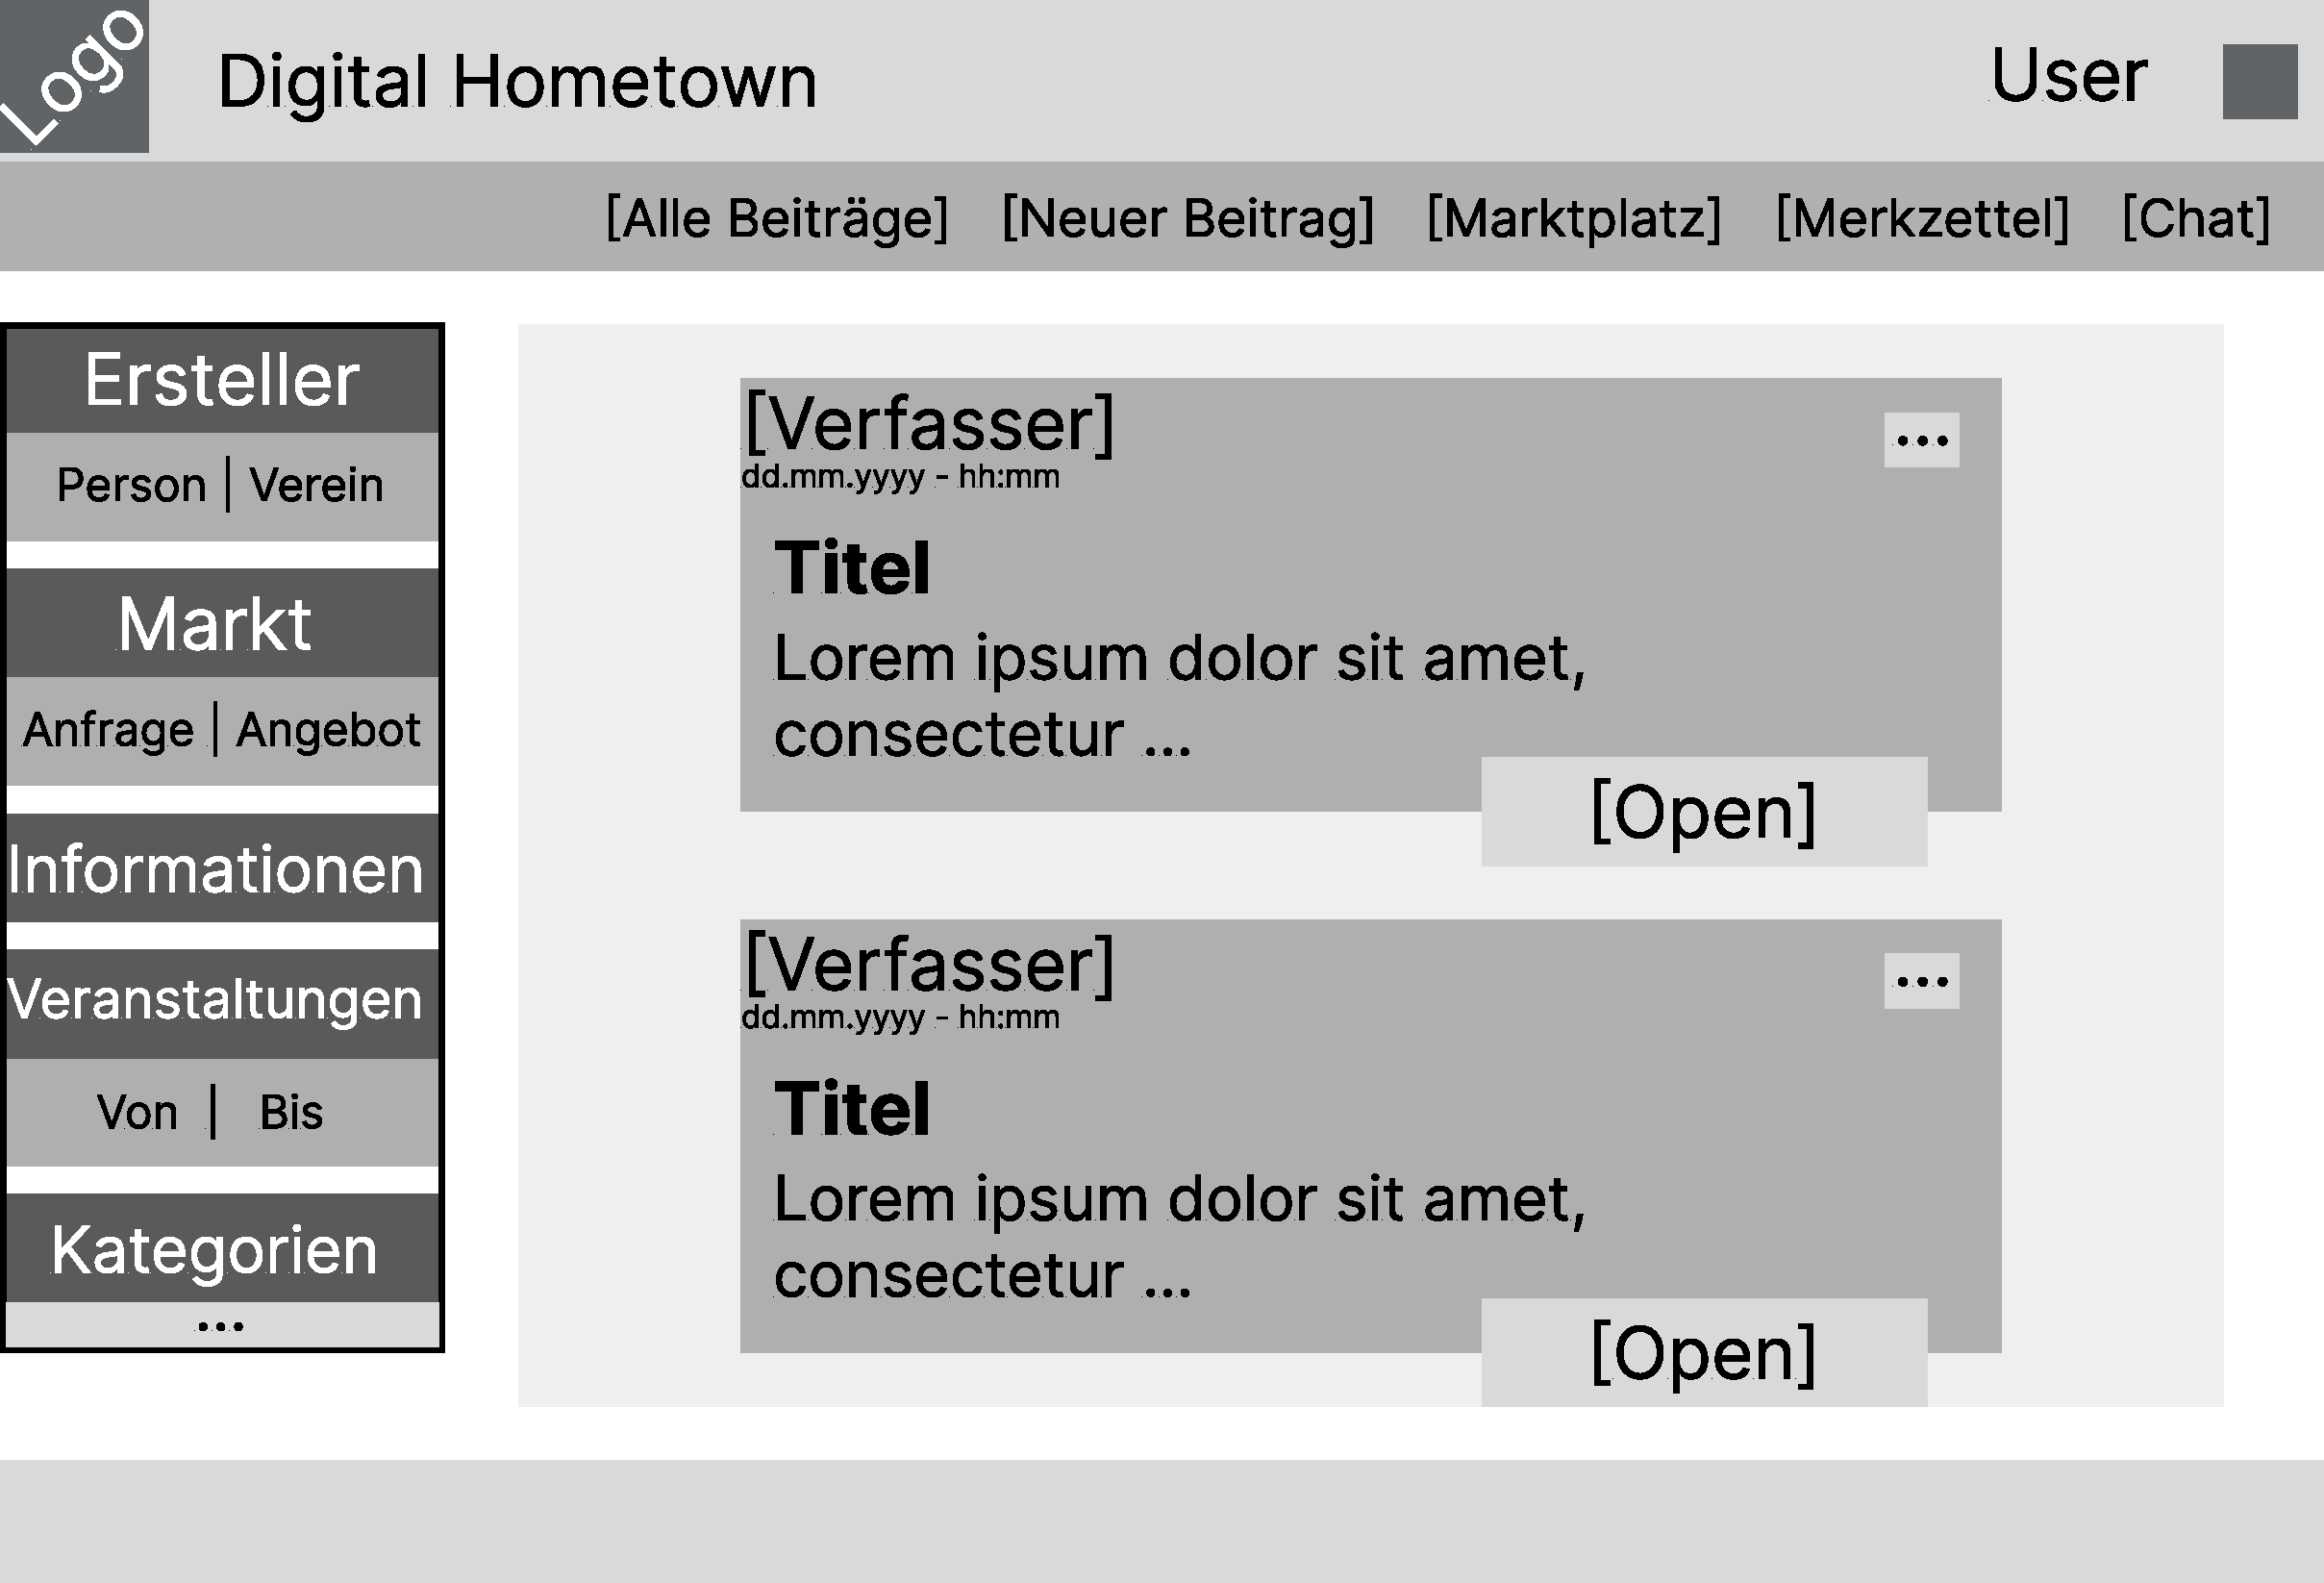
\includegraphics[page=1, width=1\textwidth]{figures/jan/wire_example.pdf}
        \caption[Marktplatz (DHT)]{Marktplatz (DHT)}
        \label{fig:image}
    \end{minipage}
\end{figure}


% \section{Usabilityanalyse}
% \label{sec:usabilityanalysis}

\section{Umfrage zur Digital-Hometown-Plattform}
\label{sec:umfrage}

Um die Plattform „Digital Hometown“ oder auch im Dokument als „Digital Dahoam“ tituliert optimal auf den Kunden auszurichten wurde im Folgenden eine Kurze Umfrage ins Leben gerufen um die Ansicht des Teams und des Kunden mit der realen Zielgruppe abzugleichen. Der Fragenkatalog wurde von mehr als 20 Personen unterschiedlichen Alters beantwortet und im Anschluss ausgewertet.

\subsection{Fragensammlung}

Neben den bereits entworfenen Personas wurde sich zu einem späteren Zeitpunkt des Projekts für die Durchführung einer Umfrage entschieden, mit dem Ziel die Bedürfnisse der Zielgruppe bestmöglich abzudecken. Hierfür wurde ein Fragebogen erstellt, bestehend aus 14 Aufgaben, welcher digital auszufüllen war. Neben einer kurzen Angabe des Alters wurden im Folgenden Präferenzen abgefragt bei der Benutzung und Bedienung einer digitalen Plattform. Ebenso wurde Inhalt somit priorisiert bzw. Features aus einer weiteren Sichtweise betrachtet. Auch Usability-Seitig wurden Anregungen entgegengenommen. Die Fragen selbst wurde als Team gemeinsam gesammelt.

\subsection{Auswertung}

Nach Abschluss der Umfrage nach einer halbwegs repräsentativen Anzahl an Teilnehmer wurden die Ergebnisse ausgewertet. Im Folgenden werden die Antworten je Fragestellung teilweise als Kreisdiagramm aber auch als Balkendiagramm dargestellt, je nach Themengebiet. Aus den gewonnenen Erkenntnissen wurden für die kommenden Sprints Themen und Features neu priorisiert und ebenso Fragestellung innerhalb der Umsetzung geklärt. Die Ergebnisse und die Wichtigkeit dieser Umfrage zeigt sich in der finalen Qualität der Homepage und des positiven Feedbacks seitens Kunde und Nutzer.

\begin{figure}[!htb]
    \centering
    \includegraphics[width=1\textwidth]{figures/daniel/Bild-3.png}
    \caption[shortcaption]{Altersverteilung Umfrage}
    \label{fig:bild3}
\end{figure}

\begin{figure}[!htb]
    \centering
    \includegraphics[width=1\textwidth]{figures/daniel/Bild-4.png}
    \caption[shortcaption]{Inhalte Marktplatz Umfrageergebnis}
    \label{fig:bild4}
\end{figure}

\begin{figure}[!htb]
    \centering
    \includegraphics[width=1\textwidth]{figures/daniel/Bild-5.png}
    \caption[shortcaption]{Inhalte Benutzerprofil Umfrageergebnis}
    \label{fig:bild5}
\end{figure}

\begin{figure}[!htb]
    \centering
    \includegraphics[width=1\textwidth]{figures/daniel/Bild-6.png}
    \caption[shortcaption]{Hauptübersicht Umfrageergebnis}
    \label{fig:bild6}
\end{figure}

\begin{figure}[!htb]
    \centering
    \includegraphics[width=1\textwidth]{figures/daniel/Bild-7.png}
    \caption[shortcaption]{Inhalte Vereinsseite Umfrageergebnis}
    \label{fig:bild7}
\end{figure}

\begin{figure}[!htb]
    \centering
    \includegraphics[width=1\textwidth]{figures/daniel/Bild-8.png}
    \caption[shortcaption]{Navigation Umfrageergebnis}
    \label{fig:bild8}
\end{figure}

\begin{figure}[!htb]
    \centering
    \includegraphics[width=1\textwidth]{figures/daniel/Bild-9.png}
    \caption[shortcaption]{Kalender Umfrageergebnis}
    \label{fig:bild9}
\end{figure}

\begin{figure}[!htb]
    \centering
    \includegraphics[width=1\textwidth]{figures/daniel/Bild-10.png}
    \caption[shortcaption]{Merkbereich Umfrageergebnis}
    \label{fig:bild10}
\end{figure}

\begin{figure}[!htb]
    \centering
    \includegraphics[width=1\textwidth]{figures/daniel/Bild-11.png}
    \caption[shortcaption]{Benutzerverifizierung Umfrageergebnis}
    \label{fig:bild11}
\end{figure}

\begin{figure}[!htb]
    \centering
    \includegraphics[width=1\textwidth]{figures/daniel/bild-12.png}
    \caption[shortcaption]{Wichtigkeit Wohnort Umfrageergebnis}
    \label{fig:bild12}
\end{figure}

\begin{figure}[!htb]
    \centering
    \includegraphics[width=1\textwidth]{figures/daniel/bild-13.png}
    \caption[shortcaption]{Kontaktiermöglichkeit Umfrageergebnis}
    \label{fig:bild13}
\end{figure}

\begin{figure}[!htb]
    \centering
    \includegraphics[width=1\textwidth]{figures/daniel/bild-14.png}
    \caption[shortcaption]{Beitragserstellung Umfrageergebnis}
    \label{fig:bild14}
\end{figure}

\begin{figure}[!htb]
    \centering
    \includegraphics[width=1\textwidth]{figures/daniel/bild-15.png}
    \caption[shortcaption]{Funktionen Beiträge Umfrageergebnis}
    \label{fig:bild15}
\end{figure}

\begin{figure}[!htb]
    \centering
    \includegraphics[width=1\textwidth]{figures/daniel/bild-16.png}
    \caption[shortcaption]{Chat Umfrageergebnis}
    \label{fig:bild16}
\end{figure}